\documentclass[a4paper,12pt]{article}
\usepackage[utf8]{inputenc}
\usepackage[T2A]{fontenc}
\usepackage[english, russian]{babel}
\usepackage[left=2cm, right=2cm, top=2cm, bottom=2cm]{geometry}
\usepackage{graphicx}
\usepackage{float}
\usepackage{wrapfig}
\usepackage{tikz}
\usepackage{amsmath, amsfonts, amssymb}
\usepackage{hyperref}
\hypersetup{
    pdfborder=0 0 0, 
    pdfstartview=FitH, 
    linkcolor=blue, 
    urlcolor=blue, 
    colorlinks=true}

\usepackage{listings}
\lstdefinestyle{codestyle}{
    backgroundcolor=\color{gray!10},
    commentstyle=\color{green!50!black},
    keywordstyle=\color{blue!80!black},
    stringstyle=\color{red!50!black},
    numberstyle=\tiny\color{gray},
    basicstyle=\ttfamily\footnotesize,
    breaklines=true,
    captionpos=b,
    numbers=left,
    numbersep=5pt,
    showstringspaces=false,
    tabsize=2
}
\lstset{style=codestyle}

\usepackage{mdframed}
\newmdenv[
  leftmargin = 0.5em,
  skipabove = 0.5em,
  skipbelow = 0.5em,
  linewidth = 1pt,
  rightline = false,
  topline = false,
  bottomline = false
]{quotebox}

\begin{document}

\begin{titlepage}
    \centering
    {\large Федеральное государственное автономное образовательное учреждение\par}
    {\large высшего образования\par}
    {\bfseries САНКТ-ПЕТЕРБУРГСКИЙ НАЦИОНАЛЬНЫЙ ИССЛЕДОВАТЕЛЬСКИЙ УНИВЕРСИТЕТ ИТМО\par}
    {\bfseries Факультет систем управления и робототехники\par}
    \vfill
    {\Large \bfseries Лабораторная работа №5\par}
    {\Large \bfseries Задачи №1521, 1628, 1650\par}
    \vfill
    
    \begin{flushright}
        Студент: Сайфуллин Д.Р. \\
        Поток: АиСД R23 1.3 \\
        Преподаватель: Тропченко А.А.
    \end{flushright}
    \vfill
    Санкт-Петербург \\
    2025 г.
\end{titlepage}

\section*{Задача №1521. Военные учения 2}
В соответствии с этой схемой учения делятся на $N$ раундов, в течение которых $N$ солдат, последовательно пронумерованных от $1$ до $N$, маршируют друг за другом по кругу, т.е. первый следует за вторым, второй за третьим, ..., $(N-1)$-й за $N$-м, а $N$-й за первым. В каждом раунде очередной солдат выбывает из круга и идёт чистить унитазы, а оставшиеся продолжают маршировать. В очередном раунде выбывает солдат, марширующий на $K$ позиций впереди выбывшего на предыдущем раунде. В первом раунде выбывает солдат с номером $K$.\\[0.5em]
Разумеется, г-н Шульман не питал никаких надежд на то, что солдаты в состоянии сами определить очерёдность выбывания из круга. «Эти неучи даже траву не могут ровно покрасить», – фыркнул он и отправился за помощью к прапорщику Шкурко.\\[1em]
\textbf{Исходные данные:}
\begin{quotebox}
    Единственная строка содержит целые числа $N$ $(1 \leq N \leq 10^5)$ и $K$ $(1 \leq K \leq N)$.
\end{quotebox}
\textbf{Результат:}
\begin{quotebox}
    Вывести через пробел номера солдат в порядке их выбывания из круга.
\end{quotebox}
\subsection*{Рабочий код}
\begin{lstlisting}[language=python]
def update_s(bit, i, delta):
    n = len(bit) - 1
    while i <= n:
        bit[i] += delta
        i += i & -i

def find_solder(bit, k):
    n = len(bit) - 1
    pos = 0
    pw = 1 << (n.bit_length() - 1)
    while pw:
        nxt = pos + pw
        if nxt <= n and bit[nxt] < k:
            k -= bit[nxt]
            pos = nxt
        pw >>= 1
    return pos + 1

def main():
    n, k = map(int, input().split())

    bit = [0] * (n + 1)
    for i in range(1, n+1):
        update_s(bit, i, 1)

    result = []
    rem = n
    cur = k

    while rem:
        cur = (cur - 1) % rem + 1 
        idx = find_solder(bit, cur)
        result.append(idx)
        update_s(bit, idx, -1)
        rem -= 1
        cur += k - 1     

    print(*result)

if __name__ == "__main__":
    main()
\end{lstlisting}
\subsection*{Объяснение алгоритма}
Этот алгоритм использует следующую идею: храним «живых» солдат как единицы в масиве, далее находим $k$-го по счёту оставшегося (бинарным подъёмом по префиксным суммам) и удаляем его (обнуляем в массиве), и так повторяем $n$ раз.

\newpage
\section*{Задача №1628. Белые полосы}
У каждого неудачника в жизни бывают не только чёрные, но и белые полосы. Марсианин Вась‑Вась отмечает в календаре, представляющем собой таблицу $m \times n$, те дни, когда ему ужасно не везло. Если Вась‑Вась не повезло в $j$-й день $i$-й недели, то он закрашивает ячейку таблицы ($i\, j$) в чёрный цвет. Все незакрашенные ячейки в таблице имеют белый цвет.\\[0.5em]
Будем называть отрезками жизни прямоугольники размером \(1 \times l\) либо \(l \times 1\). Белыми полосами Вась‑Вась считает все максимальные по включению белые отрезки таблицы. А сможете ли вы определить, сколько всего белых полос было в жизни Вась‑Вася?\\[1em]

\textbf{Исходные данные:}
\begin{quotebox}
    Первая строка содержит целые числа $m,\;n,\;k \quad(1 \le m,n \le 30000,\;0 \le k \le 60000)$, где \(m\) и \(n\) — размеры календаря, а \(k\) — количество неудачных дней в жизни Вась‑Вася. В следующих \(k\) строках перечислены неудачные дни в виде пар $(x_i, y_i)$, где \(x_i\) — номер недели, к которой относится неудачный день, а \(y_i\) — номер дня в этой неделе $(1 \le x_i \le m;\;1 \le y_i \le n)$. Описание каждого неудачного дня встречается только один раз.
\end{quotebox}
\textbf{Результат:}
\begin{quotebox}
    Выведите число белых полос в жизни Вась-Вася.
\end{quotebox}
\subsection*{Рабочий код}
\begin{lstlisting}[language=python]
def main():
    m, n, k = map(int, input().split())

    rows = [[] for _ in range(m+1)]
    cols = [[] for _ in range(n+1)]
    for _ in range(k):
        x, y = map(int, input().split())
        rows[x].append(y)
        cols[y].append(x)

    for i in range(1, m+1):
        rows[i].sort()
    for j in range(1, n+1):
        cols[j].sort()

    countH = 0
    singleH = []
    for i in range(1, m+1):
        last = 0
        for y in rows[i]:
            gap = y - last - 1
            if gap >= 2:
                countH += 1
            elif gap == 1:
                singleH.append((i, last+1))
            last = y
        gap = n - last
        if gap >= 2:
            countH += 1
        elif gap == 1:
            singleH.append((i, last+1))

    countV = 0
    singleV = []
    for j in range(1, n+1):
        last = 0
        for x in cols[j]:
            gap = x - last - 1
            if gap >= 2:
                countV += 1
            elif gap == 1:
                singleV.append((last+1, j))
            last = x
        gap = m - last
        if gap >= 2:
            countV += 1
        elif gap == 1:
            singleV.append((last+1, j))

    setH1 = set(singleH)
    isolated = 0
    for coord in singleV:
        if coord in setH1:
            isolated += 1

    print(countH + countV + isolated)

if __name__ == "__main__":
    main()
\end{lstlisting}
\subsection*{Объяснение алгоритма}
Для каждой строки находим «пробелы» между чёрными ячейками и считаем если пробел $\geq 2$, это новая горизонтальная белая полоса, инече это единичная полоса, но она станет <<максимальной>> только если нет более длинной вертикальной. Аналогично для каждого столбца считаем вертикальные белые полосы длины $\geq 2$ и запоминаем единичные фрагменты. Единичные фрагменты считаем окончательно только если они встречаются и среди горизонтальных одиночек, и среди вертикальных (то есть не содержатся ни в горизонтальной, ни в вертикальной полосах длинее 1). Сумма больших горизонтальных + больших вертикальных + изолированных даёт общее число максимальных белых полос.

\newpage
\section*{Задача №1650. Миллиардеры}
Возможно, вы знаете, что из всех городов мира больше всего миллиардеров живёт в Москве. Но, поскольку работа миллиардера подразумевает частые перемещения по всему свету, в определённые дни какой-то другой город может занимать первую строчку в таком рейтинге. Ваши приятели из ФСБ, ФБР, MI5 и Шин Бет скинули вам списки перемещений всех миллиардеров за последнее время. Ваш работодатель просит посчитать, сколько дней в течение этого периода каждый из городов мира был первым по общей сумме денег миллиардеров, находящихся в нём.\\[1em]
\textbf{Исходные данные:}
\begin{quotebox}
    В первой строке записано целое число $n$ — количество миллиардеров ($1 \leq n \leq 10000$). В каждой из следующих $n$ строк записаны данные на определённого человека: его имя, название города, где он находился в первый день данного периода, и размер состояния. В следующей строке записаны целые числа $m$ и $k$ — количество дней, о которых есть данные, и количество зарегистрированных перемещений миллиардеров соответственно ($1 \leq m \leq 50000$; $0 \leq k \leq 50000$). В следующих $k$ строках записан список перемещений в формате: номер дня (от 1 до $m - 1$), имя человека, название города назначения. Вы можете считать, что миллиардеры путешествуют не чаще одного раза в день и что они отбывают поздно вечером и прибывают в город назначения рано утром следующего дня. Список упорядочен по возрастанию номера дня. Все имена и названия городов состоят не более чем из 20 латинских букв, регистр букв имеет значение. Состояния миллиардеров лежат в пределах от 1 до 100 миллиардов.
\end{quotebox}
\textbf{Результат:}
\begin{quotebox}
    В каждой строке должно содержаться название города и, через пробел, количество дней, в течение которых этот город лидировал по общему состоянию миллиардеров, находящихся в нём. Если таких дней не было, пропустите этот город. Города должны быть отсортированы по алфавиту (используйте обычный порядок символов: ABC...Zabc...z).
\end{quotebox}
\subsection*{Рабочий код}
\begin{lstlisting}[language=python]
import heapq
from collections import defaultdict

def main():
    n = int(input())
    person_city = {}
    person_money = {}
    all_cities = set()

    for _ in range(n):
        name, city, w_s = input().split()
        w = int(w_s)
        person_city[name] = city
        person_money[name] = w
        all_cities.add(city)

    m, k = map(int, input().split())
    events = []
    for _ in range(k):
        d_s, pname, dest = input().split()
        d = int(d_s)
        events.append((d, pname, dest))
        all_cities.add(dest)
    events.sort(key=lambda x: x[0])

    city_sum = {city: 0 for city in all_cities}
    for name, city in person_city.items():
        city_sum[city] += person_money[name]

    sum_count = defaultdict(int)
    sum_cities = defaultdict(set)
    maxheap = []

    for city, s in city_sum.items():
        sum_count[s] += 1
        sum_cities[s].add(city)
    for s in sum_count:
        heapq.heappush(maxheap, -s)

    def get_top_sum():
        while maxheap:
            s = -maxheap[0]
            if sum_count[s] > 0:
                return s
            heapq.heappop(maxheap)
        return 0

    city_days = defaultdict(int)
    prev_day = 1
    idx = 0
    L = len(events)

    while idx < L:
        d, _, _ = events[idx]
        span = d - prev_day + 1
        if span > 0:
            top = get_top_sum()
            if sum_count[top] == 1:
                leader = next(iter(sum_cities[top]))
                city_days[leader] += span

        while idx < L and events[idx][0] == d:
            _, pname, dest = events[idx]
            w = person_money[pname]
            old = person_city[pname]

            old_s = city_sum[old]
            sum_count[old_s] -= 1
            sum_cities[old_s].remove(old)
            city_sum[old] = old_s - w
            new_old_s = old_s - w
            sum_count[new_old_s] += 1
            sum_cities[new_old_s].add(old)
            heapq.heappush(maxheap, -new_old_s)

            prev_s2 = city_sum.get(dest, 0)
            sum_count[prev_s2] -= 1
            sum_cities[prev_s2].discard(dest)
            city_sum[dest] = prev_s2 + w
            new_s2 = prev_s2 + w
            sum_count[new_s2] += 1
            sum_cities[new_s2].add(dest)
            heapq.heappush(maxheap, -new_s2)

            person_city[pname] = dest
            idx += 1

        prev_day = d + 1

    if prev_day <= m:
        span = m - prev_day + 1
        if span > 0:
            top = get_top_sum()
            if sum_count[top] == 1:
                leader = next(iter(sum_cities[top]))
                city_days[leader] += span

    for city in sorted(city_days):
        days = city_days[city]
        if days > 0:
            print(city, days)

if __name__ == "__main__":
    main()
\end{lstlisting}
\subsection*{Объяснение алгоритма}
Для каждого города \(c\) поддерживаем текущую сумму состояний миллиардеров. События (перемещения) упорядочены по дню \(d\). Пусть \(\mathit{prev\_day}\) --- день предыдущего события плюс один. Перед обработкой всех событий дня \(d\) начисляем отрезок дней тому городу, который единолично обладает максимальной суммой. Затем для каждого перемещения миллиардера с весом \(w\) из города \(u\) в \(v\) обновляем города, соответствующим образом уменьшая/увеличивая сумму и множества городов, а также добавляя новые значения в кучу. После всех событий обрабатываем оставшийся отрезок аналогичным образом.

\section*{Статус проверки}
\begin{figure}[H]
    \centering
    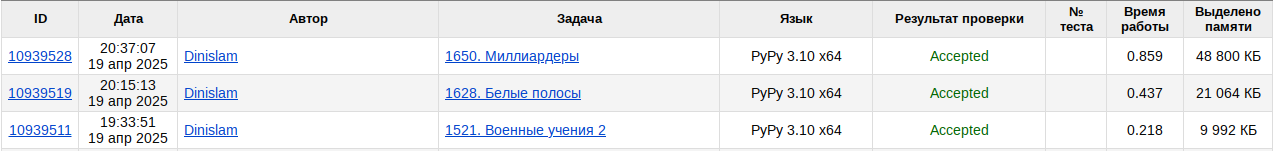
\includegraphics[width=1\textwidth]{check_status.png}
    \caption{Результат проверки}
\end{figure}

\end{document}

